\section{Datos a analizar}

De cara a realizar esta práctica se utilizarán datos extraídos de la red social Twitter. En concreto, se utilizarán los tweets de la cuenta \href{https://twitter.com/CosmereQuotes}{CosmereQuotes}, una cuenta que publica citas de los libros del Cosmere, universo de fantasía donde se ambientan los libros del autor Brandon Sanderson.

He decidido utilizar estos tweets como documentos debido a que he leído los libros y por lo tanto tengo información sobre los documentos, siendo esto una ventaja a la hora de analizar los resultados y saber si estos son coherentes.

\section{Lectura de los datos}

Para realizar la lectura de datos utilizaremos el plugin KNIME Twitter Connectors. Este plugin nos permite utilizar los nodos Twitter API Connector y Twitter Search.

Con el nodo Twitter API Connector introduciremos los datos necesarios para realizar la conexión a la API de Twitter, y una vez estemos conectados, pasamos al nodo Twitter Search.

El nodo Twitter Search nos permite definir la búsqueda que realizaremos. En este caso no buscaremos palabras concretas, utilizaremos el parámetro \texttt{from} para definir de que cuenta se van a obtener los tweets. También podemos establecer el número de tweets que vamos a obtener (aunque como veremos, debido a las limitaciones de la API de Twitter obtendremos un número limitado de tweets), así como la información a almacenar de cada tweet.

\begin{figure}[H]
	\centering
	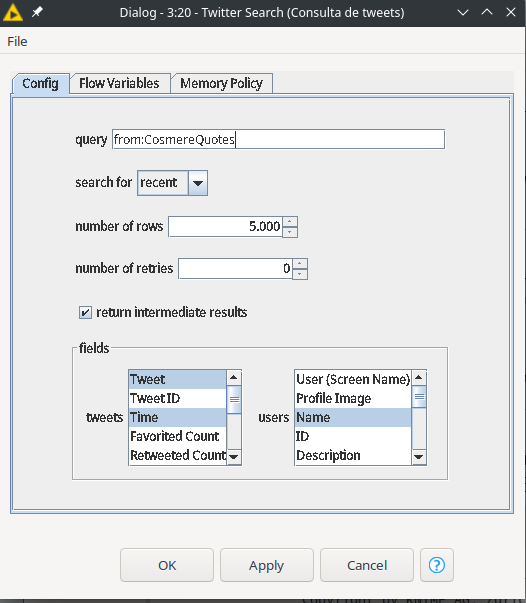
\includegraphics[scale = 0.6]{busqueda_TW.png}
	\caption{Configuración del nodo Twitter Search.}
	\label{fig:busqueda_TW}
\end{figure}

Tras ejecutar este nodo, obtenemos los siguientes datos:

\begin{figure}[H]
	\centering
	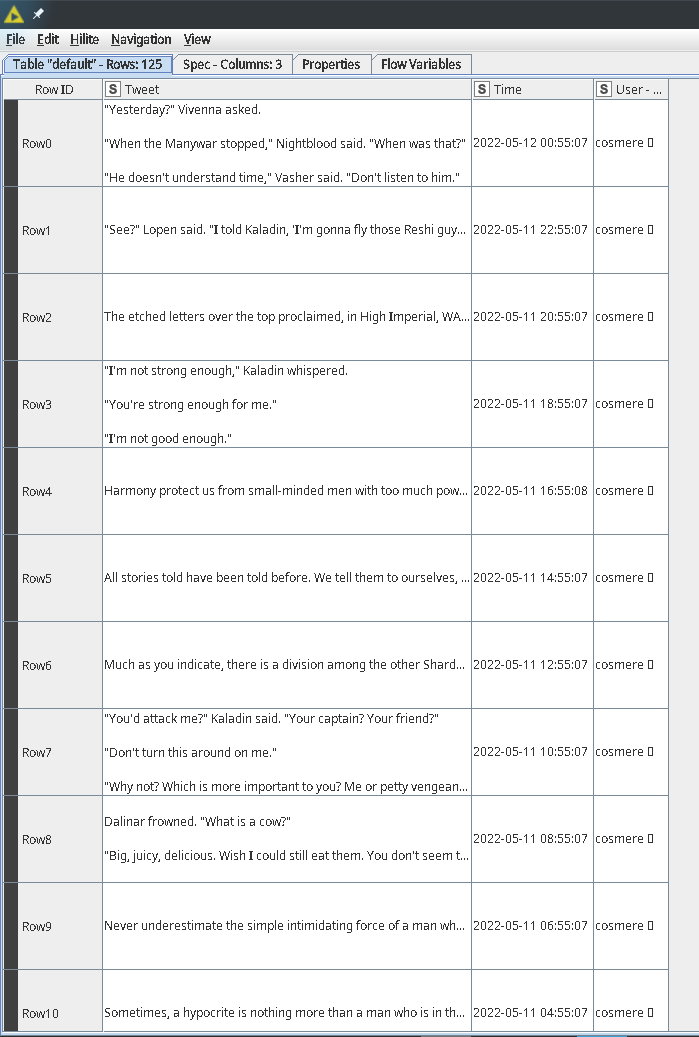
\includegraphics[scale = 0.6]{entrada_datos.png}
	\caption{Datos obtenidos por el nodo Twitter Search.}
	\label{fig:entrada_datos}
\end{figure}


Como podemos ver, los tweets leídos son casillas de texto, y no documentos, por este motivo utilizaremos un nodo String to Document para convertir la columna Tweet en un documento.


\begin{figure}[H]
	\centering
	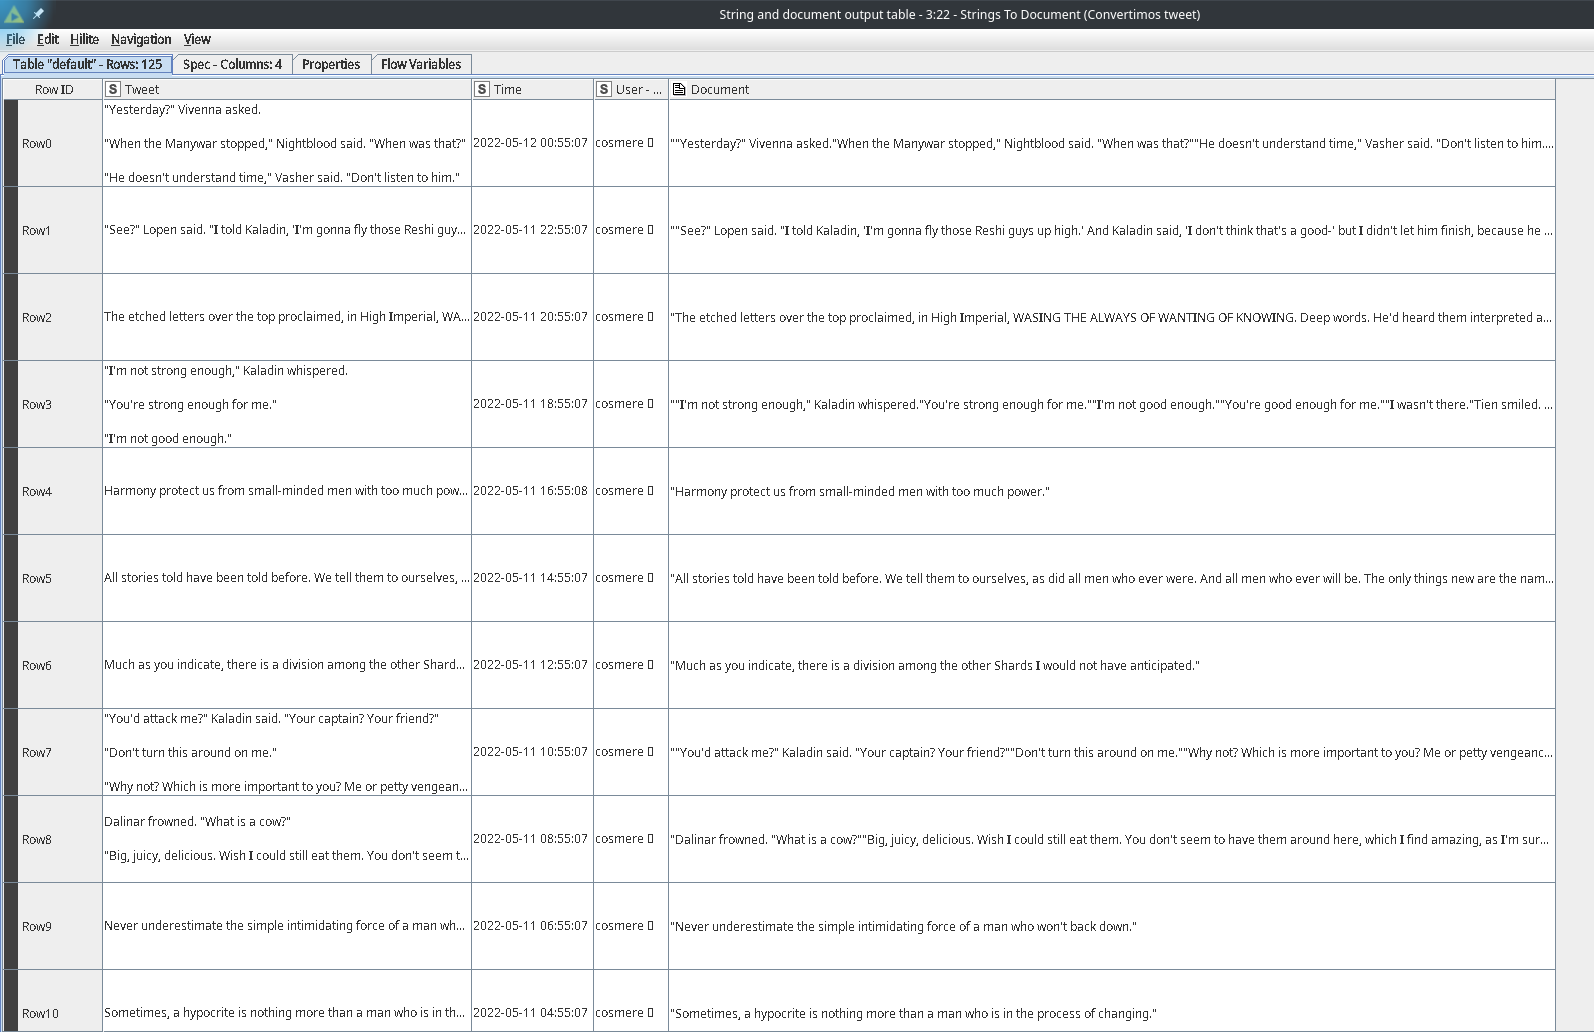
\includegraphics[width = \textwidth]{entrada_datos_documentos.png}
	\caption{Datos obtenidos por el nodo String to Document.}
	\label{fig:entrada_datos_documentos}
\end{figure}


Un detalle importante es que debido a las limitaciones de la API de Twitter contamos con tan solo los 125 tweets más recientes, y no todos los tweets de la cuenta, por lo que el número de documentos es 125.

Con esto, ya tenemos preparados los documentos con los que trabajaremos.

\section{Enriquecimiento de los documentos}

Una vez tenemos los documentos preparados podemos pasar el enriquecimiento. En este caso es muy simple, solamente se usará un nodo POS Tagger para asignar a cada termino de un documento una etiqueta que marcará los términos similares de cada documento.

\begin{figure}[H]
	\centering
	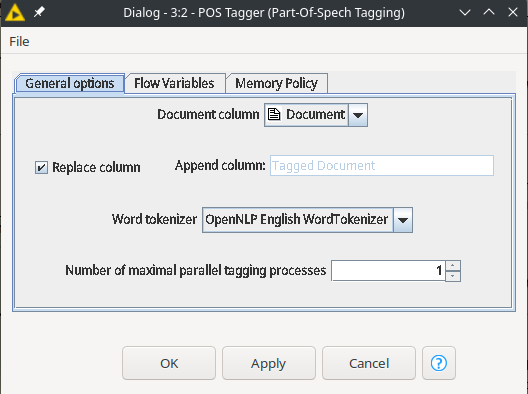
\includegraphics[scale = 0.6]{POS_tagger.png}
	\caption{Configuracion del nodo POS Tagger.}
	\label{fig:POStagger}
\end{figure}

Como los documentos utilizados son texto en inglés, se usará como tokenizador OpenNLP English WordTokenizer.


\section{Preprocesamiento}

Con respecto al preprocesamiento se han utilizado los siguientes nodos:

\begin{itemize}
	\item Punctuation Erasure: Eliminar todos los caracteres de puntuación de los documentos, como los puntos, las comas, comillas, etc.
	\item Diacritic Remover: Elimina los signos diacríticos de los documentos de entrada. Este nodo es importante en nuestro caso ya que al tratarse de documentos relacionados con literatura de fantasía existen términos que utilizan estos signos para marcar la pronunciación.
	\item N Chars Filter: Elimina todos los términos con una longitud menor a la dada, en este caso dos caracteres. Nos permite eliminar términos conectores que no aportan información.
	\item Tag Filter: Permite seleccionar términos por categorías. En nuestro caso escogeremos solo los términos que sean nombres.
	\item Porter Stemmer: Permite obtener la raíz de los términos utilizando el algoritmo de Porter. De esta forma, los términos son reducidos a su raíz.
\end{itemize}

Tras aplicar todos estos pasos a los documentos, obtenemos el siguiente resultado:

\begin{figure}[H]
	\centering
	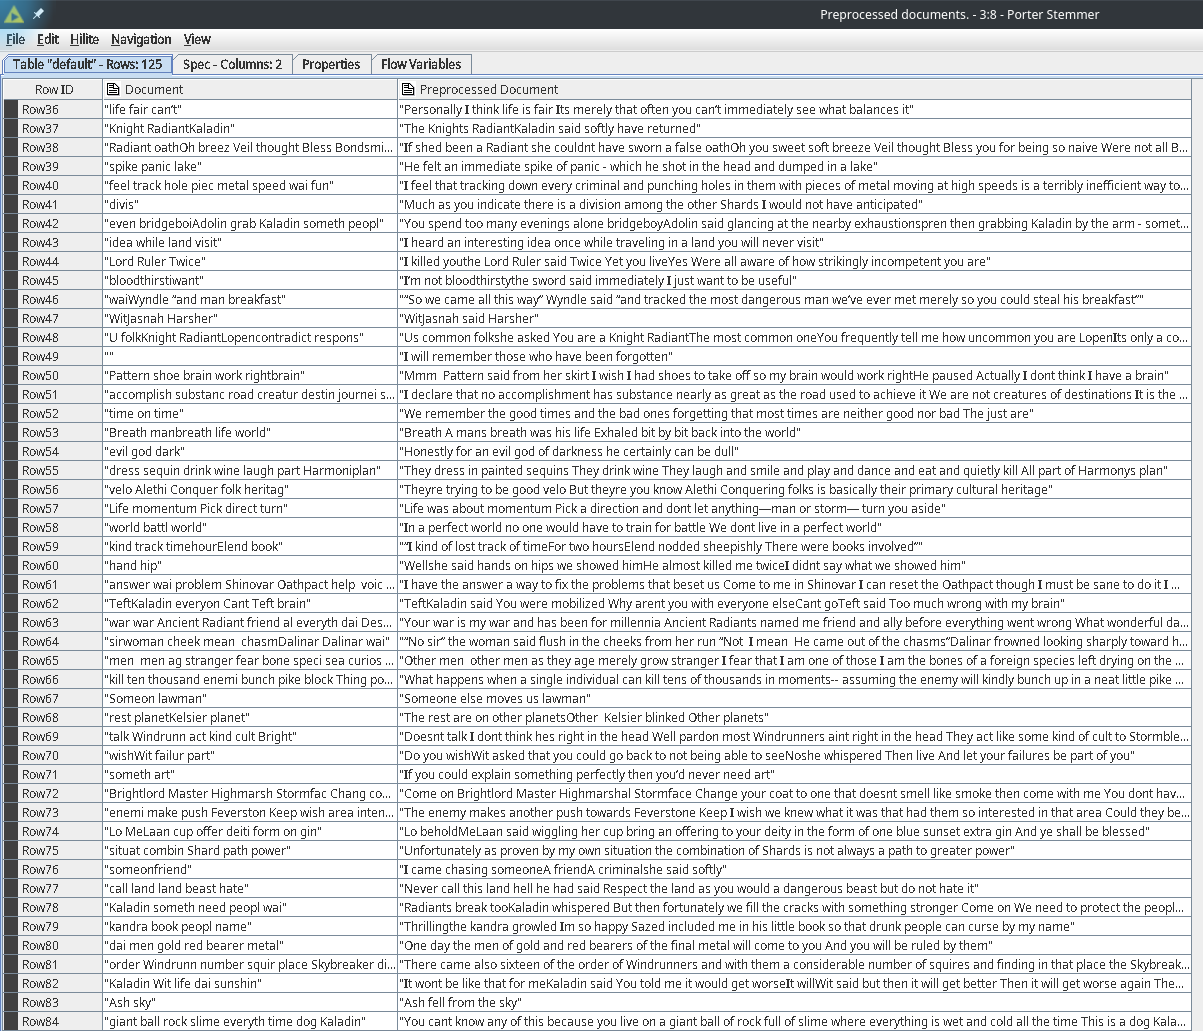
\includegraphics[width = \textwidth]{documentos_preprocesados.png}
	\caption{Documentos tras aplicar el preprocesado.}
	\label{fig:documentos_preprocesados}
\end{figure}


\section{Técnica de minería}

Para la técnica de minería se utilizará un clustering jerárquico. Para poder usar esta técnica primero tenemos que realizar la extracción de términos y transformar los documentos a una representación en la que se pueda calcular la distancia entre dos términos.

En concreto se ha usado el nodo Keygraph Keyword Extractor, con el que de cada documento extraeremos los términos considerados más importantes. Tras esto se ha usado el nodo Document Vector para transformar cada documento en un vector numérico usando como columnas los términos, una representación que si podemos usar en la técnica de minería.

Una vez estas transformaciones se ha usado el nodo Hierarchical Clustering para aplicar el clustering jerárquico, obteniendo los siguientes resultados:

\begin{figure}[H]
	\centering
	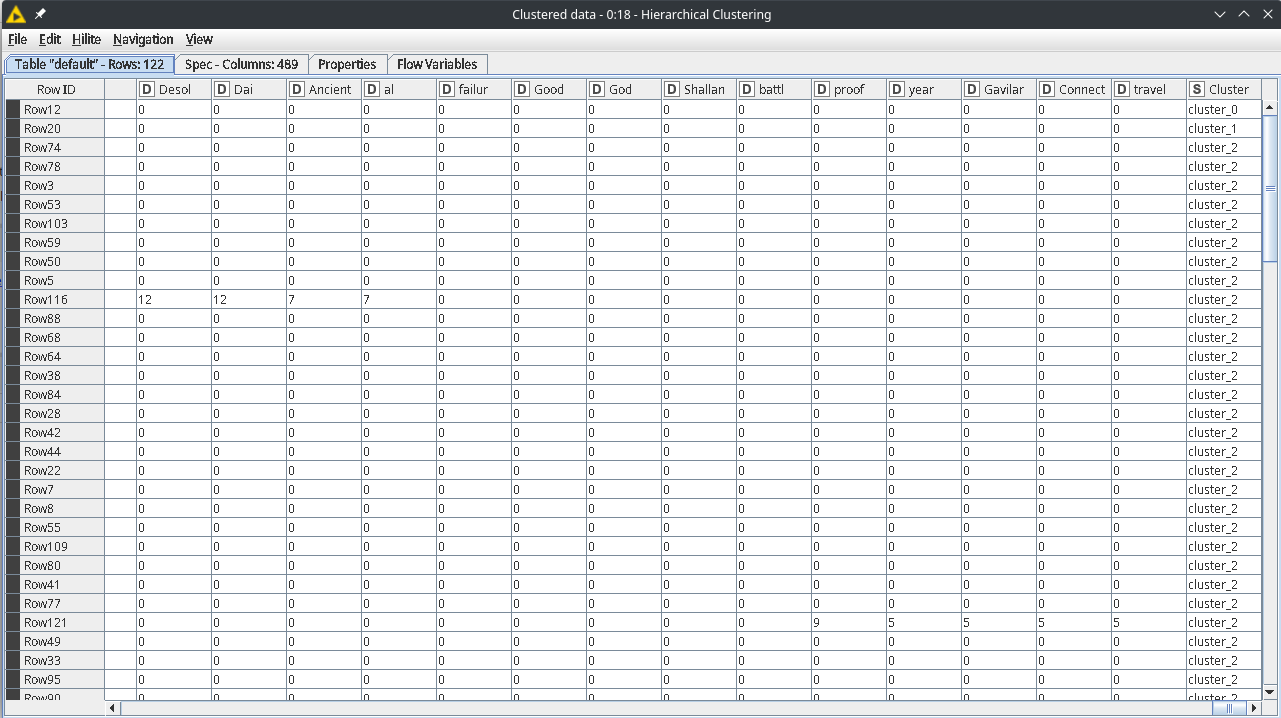
\includegraphics[width = \textwidth]{tabla_clustering.png}
	\caption{Tabla de documentos tras aplicar el clustering.}
	\label{fig:tabla_clustering}
\end{figure}

También obtenemos el siguiente dendograma:

\begin{figure}[H]
	\centering
	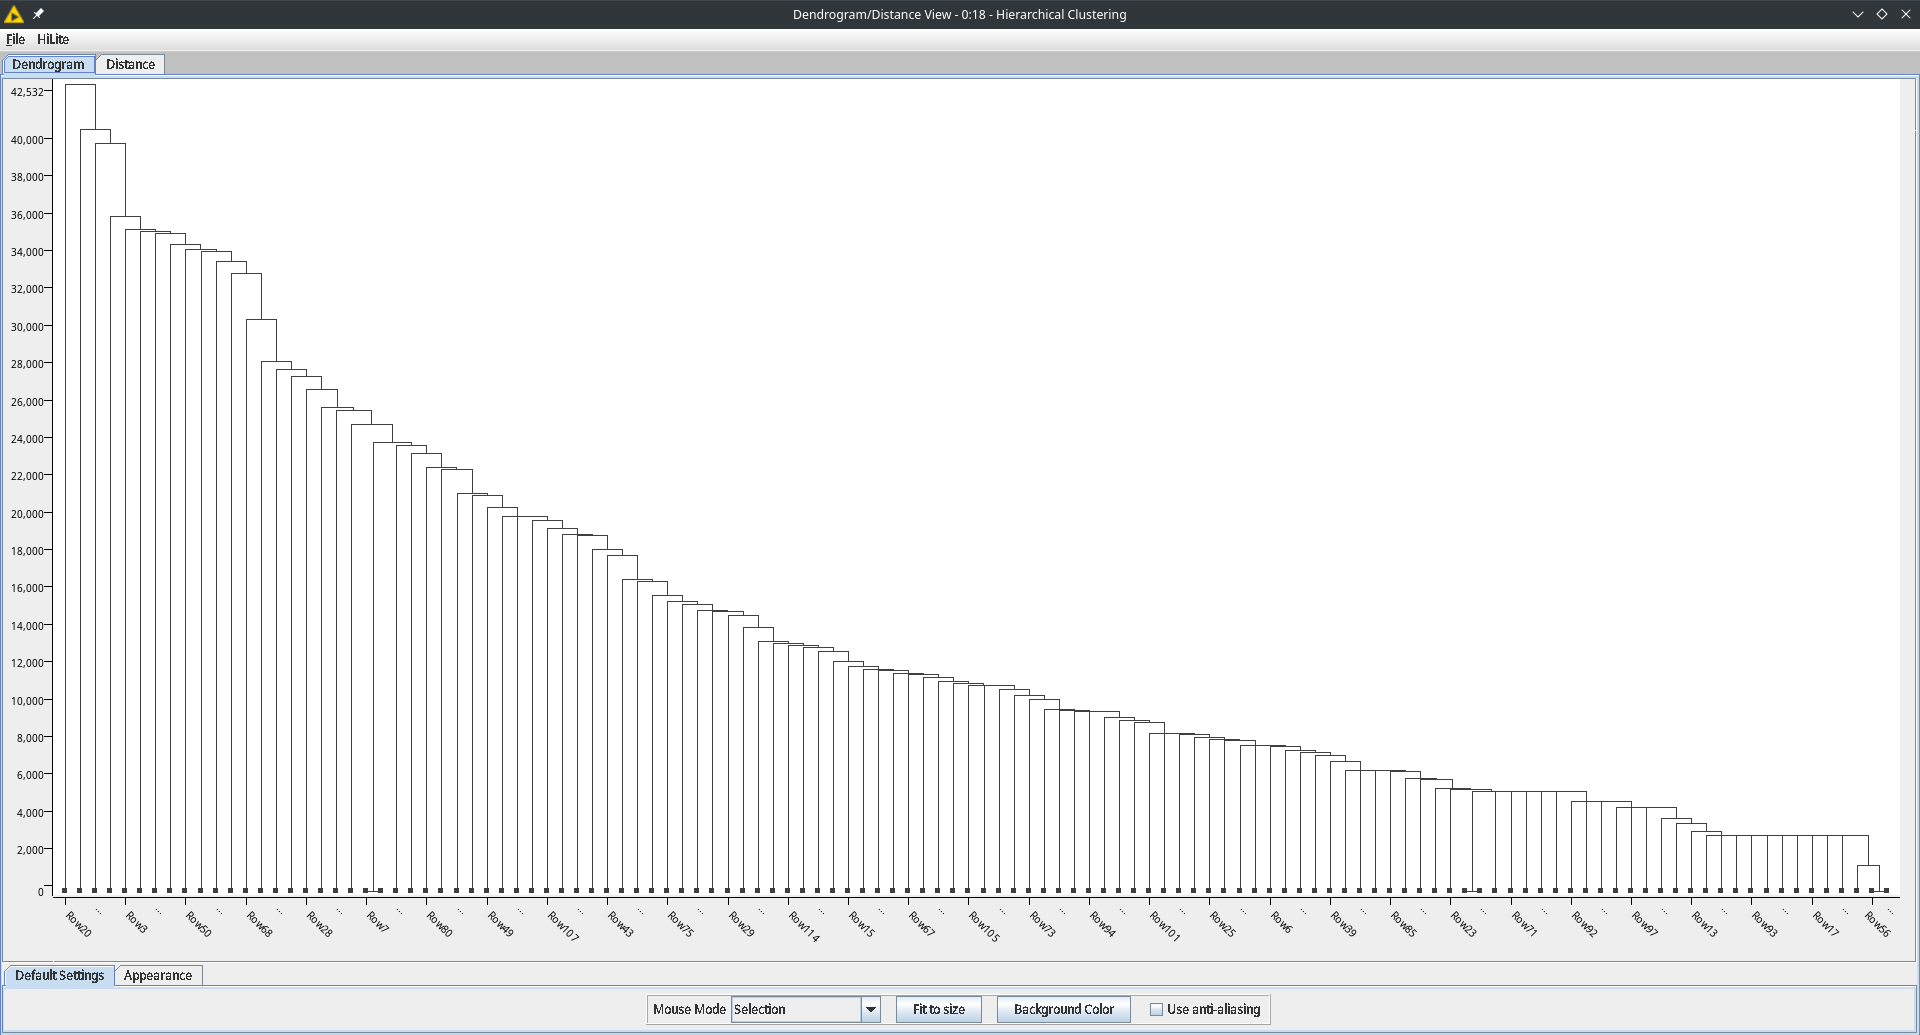
\includegraphics[width = \textwidth]{dendograma.png}
	\caption{Dendograma obtenido con el clustering.}
	\label{fig:dendograma}
\end{figure}


\section{Visualización}

Para la visualización utilizaré el nodo Tag Cloud, ya que se trata de la opción más visual y directa para ver la información extraída.

Primero, el resultado de Porter Stemmer se pasará por un nodo Bag of Words Creator, para representar los documentos como bolsas de palabras. Tras esto, se calculará la frecuencia relativa y absoluta de cada término, así como la inversa de su frecuencia, lo que usaremos para conocer las palabras de mayor relevancia para la nube de palabras. Antes de usar la nube también se aplicará un filtrado por frecuencia, para eliminar los términos que no sean relevantes. Con esto ya si aplicamos la nube de palabras, con la que obtenemos el siguiente resultado:


\begin{figure}[H]
	\centering
	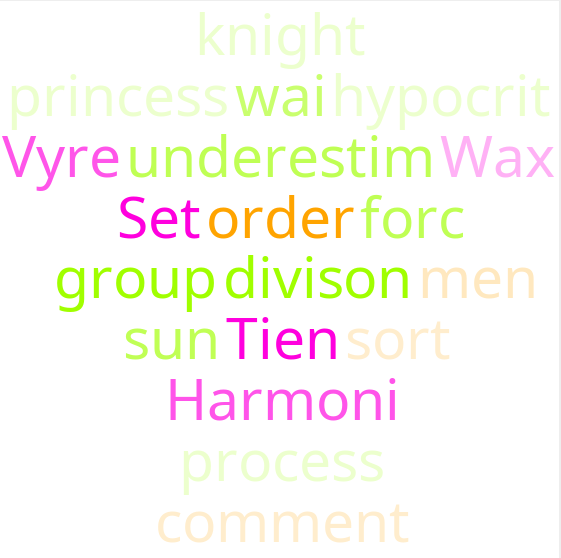
\includegraphics[scale = 0.8]{nube_palabras.png}
	\caption{Nube de palabras.}
	\label{fig:nube_palabras}
\end{figure}

Teniendo información sobre los documentos podemos ver que esta nube de palabras tiene sentido, apareciendo con bastante importancia personajes importantes de las dos principales sagas, El Archivo de las Tormentas (Vyre, Tien y Set) y Nacidos de la Bruma (Wax y Harmoni), así como términos que tienen cierta relevancia en el contexto de los libros.

\section{Workflow final}


El flujo final realizado a lo largo de la práctica es el siguiente:

\begin{figure}[H]
	\centering
	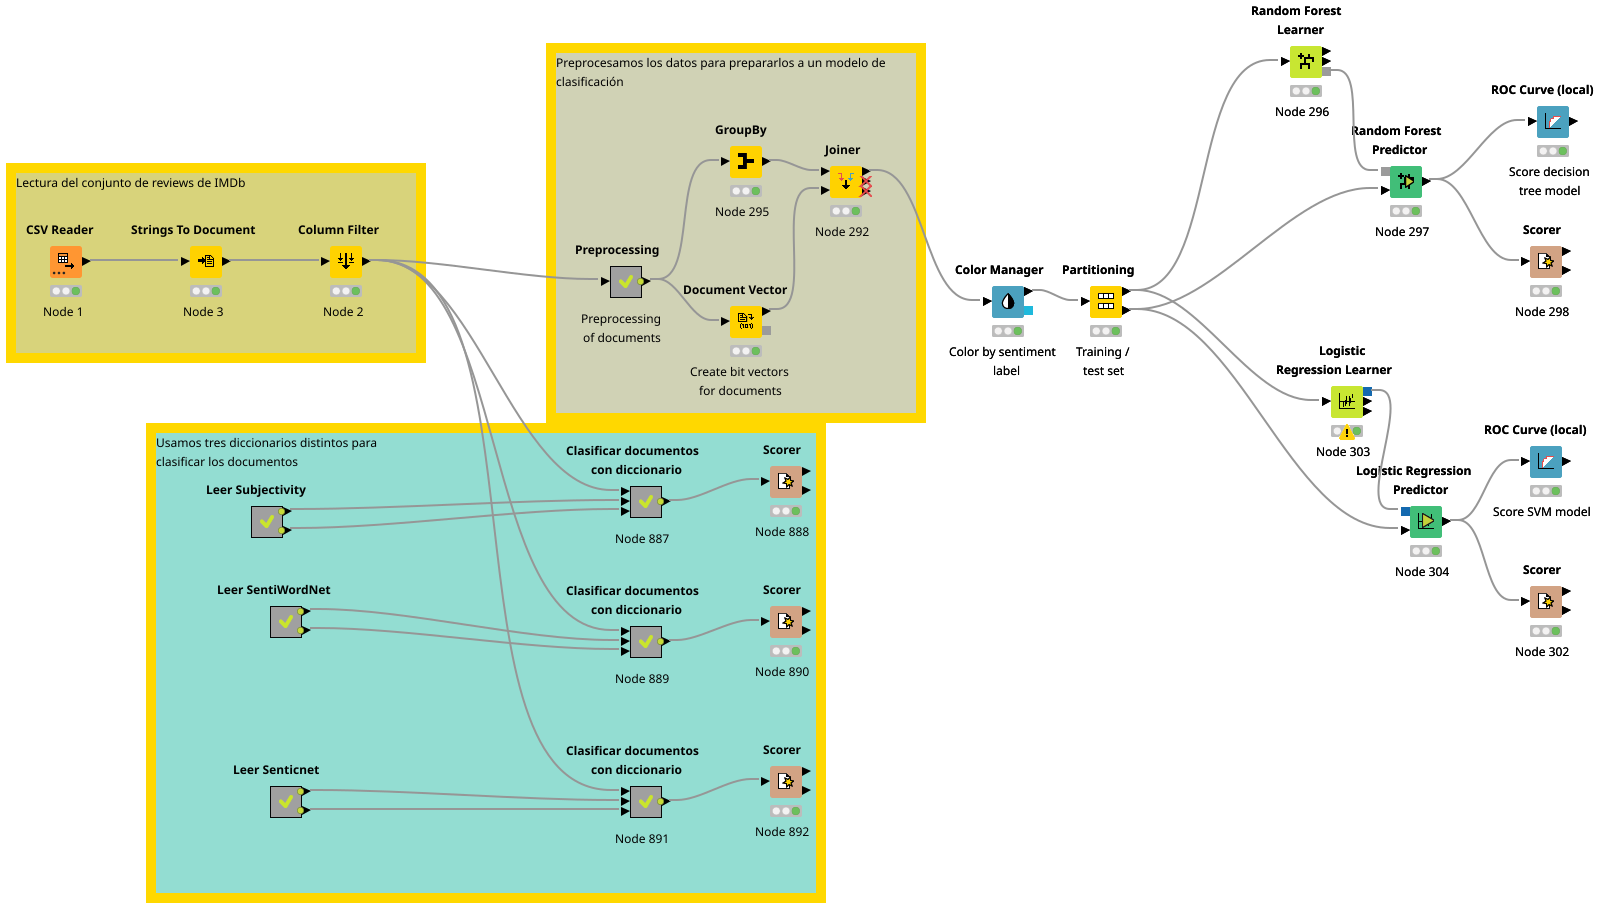
\includegraphics[width = \textwidth]{workflow_knime.png}
	\caption{Workflow final de KNIME.}
	\label{fig:workflow_knime}
\end{figure}


Como podemos ver, toda la parte de lectura y preprocesamiento es común, y simplemente difiere el flujo al aplicar tareas concretas, por lo que si quisiéramos seguir trabajando con estos datos podríamos aprovechar gran parte del flujo.
